\chapter{Computing Angle of Arrival}
If the radar has at least two transmit-receive antenna pairs, we can calculate
the angle of arrival (AoA) for the received signal from the
phase differences in the spectra, which arise from the slight differences
in range of the object from each receiving antenna.

% drawing of antenna and \delta d
\begin{figure}[h]
	\center
	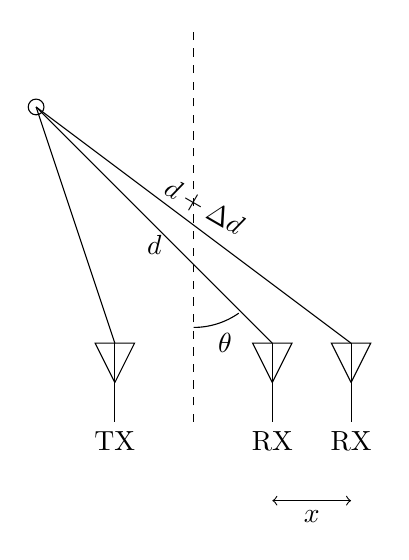
\begin{tikzpicture}
		\draw (1,0.5) -- (0.75, 1) -- (1.25, 1) -- (1,0.5);
		\draw (1, 1) -- (1,0) node[below] {RX};
		\draw (2,0.5) -- (1.75, 1) -- (2.25, 1) -- (2,0.5);
		\draw (2, 1) -- (2,0) node[below] {RX};
		\draw[<->] (1,-1) to node[below] {$x$} (2, -1);
		\draw (-1,0.5) -- (-0.75, 1) -- (-1.25, 1) -- (-1,0.5);
		\draw (-1, 1) -- (-1,0) node[below] {TX};
		\draw (-2,4) circle [radius=0.1];
		\draw (-2,4) to node[below] {$d$} (1,1);
		\draw (-2,4) to node[above, rotate=330] {$d+\Delta d$}  (2,1);
		\draw (-2,4) to (-1,1);
		\draw[dashed] (0,0) to (0,5);
		\draw (0,1.2) arc (-90:-55:1);
		\draw (0.4, 1) node {$\theta$};
	\end{tikzpicture}
	\caption{Angle of arrival problem}
	\label{fig:angle-of-arrival}
\end{figure}

\section{Geometric Estimation}
From Figure \ref{fig:angle-of-arrival}, we can derive the phase difference
between the received signals $r_1(t)$ and $r_2(t)$ at two different antennas
separated by a distance $x$. Let $d$ be the distance the received signal
$r_1(t)$ travels to reach the first antenna and $d + \Delta d$ be the distance
the reflected signal $r_2(t)$ travels to reach the second antenna
\cite{iovescu2017fundamentals}. Assuming the
radar signal is a planar wavefront, the geometry shown in Figure
\ref{fig:geometric-aoa} gives
\begin{equation}
	\Delta d = x \sin \theta. 
\end{equation}
\begin{figure}
	\center
	\begin{tikzpicture}
		\draw[dashed] (0,-0.5) to (0,6);
		\draw (2,0) to node[below] {$x$} (4,0);
		\draw (4,0) to node[above, rotate=315] {$\Delta d$} (3, 1);
		\draw (2,0) to (3, 1);
		\draw (2.8, 0.8) -- (3, 0.6) -- (3.2, 0.8);
		\draw (2.4, 0) arc (0:45:0.4) node[right] {$\theta$};
		\draw (2,0) to (-1, 3.3);
		\draw (4,0) to (-1,5);
		\draw (0,1.8) arc (-90:-45:0.4) node[below] {$\theta$};
		\draw (2,0) to (2,-0.5);
		\draw (4,0) to (4, -0.5);
	\end{tikzpicture}
	\caption{Geometric approach for estimating angle of arrival}
	\label{fig:geometric-aoa}
\end{figure}

Now, the phase difference $\Delta \phi$ is given by
\begin{equation}
	\Delta \phi = \frac{2\pi \Delta d}{\lambda}.
\end{equation}
Now, we can compute the angle of arrival $\theta$ as 
\begin{equation}
	\theta = \sin^{-1}(\frac{\lambda\Delta\phi}{2\pi x}).
\end{equation}
However, since $\Delta\phi$ depends on $\sin\theta$, our accuracy degrades for
large $\theta$, as $\sin\theta \approx \theta$ only for small $\theta$. 

As before, for the phase difference to be unambiguous, $|\Delta\phi |<\pi$, so we
find
\begin{equation}
	\frac{2\pi x}{\lambda} \sin\theta < \pi,
\end{equation}
and the maximum field of view for two TX-RX antenna pairs spaced $x$ apart is 
\begin{equation}
	\theta_{max} = \sin^{-1}(\frac{\lambda}{2x}).
\end{equation}
Clearly, the largest angular field of view for two antenna pairs with this
approach occurs when the antenna spacing is
\begin{equation}
	x = \frac{\lambda}{2},
\end{equation}
giving $\theta_{max} = \pm\frac{\pi}{2}$.

\section{Multiple Signal Classification (MUSIC)}
For multiple-input multiple-output (MIMO) FMCW radar systems, we can use more
sophisticated angle-of-arrival techniques based on subspaces. Let
us assume we have an arbitrary array of $L$ virtual transmit-receive antenna pairs, with an
array response vector $\bm{a}(\theta)$. This response vector maps the direction
of arrival $\theta$ to the signal phase shift at each of the $L$ virtual antenna
pairs. For a set of $N$ objects, we will have $N$ return signals $r(t)$
returning to the antenna array. Let $\bm{x}(t)$ be the superposition of the
signals so that \cite{bresler2017hilbert}
\begin{align}
	\bm{x}(t) &= \sum_{n=1}^N s_n(t) \bm{a}(\theta_n)\\
	&= \bm{A}(\bm{\theta})\bm{s}(t),
\end{align}
where
\begin{align}
	\bm{A}(\bm{\theta}) &= [\bm{a}(\theta_1), \bm{a}(\theta_2), \dots, \bm{a}(\theta_N)]\\
	\bm{\theta} &= [\theta_1, \theta_2, \dots, \theta_N]^T\\
	\bm{s}(t) &= [s_1(t), s_2(t), \dots, s_N(t)]^T.
\end{align}
If we sample $\bm{x}(t)$ at $M$ timesteps, we get the following matrix equation:
\begin{equation}
	\bm{X} = \bm{A}(\bm{\theta})\bm{S},
\end{equation}
where $\bm{X}$ is an $L \times M$ matrix of samples, $\bm{A}(\bm{\theta})$ is
an
$L\times N$ matrix function, and $\bm{S}$ is a $N\times M$ matrix
\begin{align}
	\bm{X} &= [\bm{x}(t_1), \bm{x}(t_2), \dots, \bm{x}(t_M)]\\
	\bm{S} &= [\bm{s}(t_1), \bm{s}(t_2), \dots, \bm{s}(t_M)].
\end{align}
Since $\bm{X}$ is the product of an $L\times N$ matrix and an $N\times M$ matrix,
we have that $rank(\bm{X}) = N$, assuming $\bm{A}(\bm{\theta})$ has full column
rank and $\bm{S}$ has full row rank. This corresponds to the number of objects
whose angular position we are trying to compute. Now, since the range space of
$\bm{X}$, $\mathcal{R}(\bm{X})$, is the same subspace as the range space of
$\bm{A}(\bm{\theta})$
\begin{equation}
	\mathcal{R}(\bm{X}) = \mathcal{R}(\bm{A}(\bm{\theta})),
\end{equation}
we can use the singular value decomposition (SVD) of $\bm{X}$ to recover
$\theta_i$. The SVD of $\bm{X}$ is given by
\begin{align}
	\bm{X} &= \bm{U} \bm{\Sigma} \bm{V}^H\\
	&= [\bm{U_s} | \bm{U_n}] \begin{bmatrix} \Sigma_s & 0 \\
	0 & \bm{0} \end{bmatrix} \bm{V}^H,
\end{align}
where the left singular vectors have been separated into those corresponding
to the nonzero singular values ($\bm{U}_s$) and those corresponding to the
zero singular values ($\bm{U}_n$). From linear algebra, we know the columns of
$\bm{U}_s$ span the signal subspace $\mathcal{R}(\bm{X})$ and the columns of
$\bm{U}_n$ span the left nullspace $\mathcal{N}{\bm{X}^H})$ of $\bm{X}$, which
is the orthogonal complement of the signal subspace \cite{meyer2000matrix}. In this context, we will
call this subspace the noise subspace
\begin{align}
	\text{span}(\bm{U_n}) &= \mathcal{N}(\bm{X}^H) \\
	&= \mathcal{R}(\bm{X})^\perp\\
	&= \mathcal{R}(\bm{A}(\bm{\theta}))^\perp.
\end{align}
Now, if we sweep $\theta \in [0, 2\pi)$, $\bm{a}(\theta)$ will lie in the left
nullspace of $\bm{X}$ when $\theta=\theta_i$, where $\theta_i$ are the desired
angles of arrival we are estimating, 
\begin{equation}
	\theta = \theta_i \iff \bm{U}_n^H \bm{a}(\theta) = 0.
\end{equation}
The multiple signal classification (MUSIC)
algorithm leverages this fact by finding the peaks in \cite{schmidt1986multiple}
\begin{equation}
	g(\theta) = \frac{1}{\|\bm{U}_n^H \bm{a}(\theta)\|^2}.
\end{equation}

%\section{ESPRIT}
